We consider the use case of a network operator migrating core infrastructure from traditional switching and routing elements to a centrally managed SDN architecture. We assume the migration process will occur in three discrete phases, with a single intermediate migration state. 


% \section{Application Case Study:}\label{subsec:approach:main}
% \chapter{Related Work}

\section{MITRE ATT\&CK Framework}\label{sec:related:mitre}

\section{MulVal Infrastructure Modeling}\label{sec:related:mulval}

\section{PKB}\label{sec:related:pkb}

\subsection{Migration Path}


\begin{figure}[ht]
\centering
\begin{subfigure}{.33\textwidth}
\includegraphics[width=\linewidth]{resource/img/ch_background/sdn_analytics/use_case_figs/mig_step_001.png}
\caption{Current}
\label{fig:current}
\end{subfigure}%
\begin{subfigure}{.33\textwidth}
\includegraphics[width=\linewidth]{content/chapters/ch_background/sdn_analytics/2/figs/use_case_figs/mig_step_002.png}
\caption{Transition}
\label{fig:trans}
\end{subfigure}%
\begin{subfigure}{.33\textwidth}
\includegraphics[width=\linewidth]{content/chapters/ch_background/sdn_analytics/2/figs/use_case_figs/mig_step_003.png}
\caption{Future}
\label{fig:future}
\end{subfigure}%
    \caption{Network migration models from current to future}
\end{figure} 


The primary network elements we consider for this analysis are \textit{Customer Edge (CE)} routers, \textit{Provider Edge (PE)} routers, and \textit{Provider Core (P)} routers. \textit{CE} routers attach to \textit{PE} routers and communicate information about the customer network  topology to the provider. \textit{PE} routers exchange routing information with other \textit{PE} routers about the networks they are attached to. \textit{PE} routers also learn from \textit{P} routers what paths are available through the provider network.  Once routing and signalling information is established, the \textit{PE} and \textit{P} routers can forward customer traffic through the provider network. In conventional networks routing and signalling information is exchanged directly between adjacent routers, whereas the controller receives this information in SDN architectures. To determine the correct path through the network, routers and switches are required to parse frame and packet headers to identify the source and destination of incoming traffic. \textit{Multi Protocol Label Switching (MPLS)}\cite{Awduche_Agogbua_1999} is used to reduce the overhead of packet processing and isolate customer traffic by applying labels on incoming packets. Labels speed up routing through core and transit networks by reducing the effort needed to process the header at each hop. We have reduced the scale and scope of the network models to capture some of the key changes in the architectures during migration while reducing overall complexity. These representative models allow us to isolate the impact of specific architecture changes on the system’s security.  %Follow on efforts to leverage existing network mapping, network management, and vulnerability scanning tools will enable automated generation of more accurate and near real time network models. This work could be incorporated into the existing security incident event management (SIEM) system for visibility into the security effects of hardware or software level changes on the network.  

The current network model depicted in Figure \ref{fig:current} captures the existing architecture elements such as distributed routing protocols and hardware and operating system level components. When customer traffic enters the Ingress Router PE1 from the customer edge CE1, access control lists are enforced to drop any packets with a destination address matching the address of the core infrastructure. Traffic flows that are not denied by the ACL are then routed through the MPLS core and forwarded to the appropriate Egress Router. In practice, the number of ACL rules maintained on each Ingress Router could exceed 100,000 entries.  

The transition state network in Figure \ref{fig:trans} retains the same logical connectivity as the current network by leveraging ACLs to restrict customer traffic. This model introduces a global SDN controller along with the supporting infrastructure to facilitate a centrally managed SDN environment. Proprietary switching hardware has been replaced by merchant silicon and the vendor specific applications that control the hardware have been abstracted and moved onto the hypervisor. The result is that, while ACLs can now be centrally managed, the attack surface of the network has increased with the addition of the SDN components.

The final network model in Figure \ref{fig:future} assumes the same underlying infrastructure as the transitional SDN model in \ref{fig:trans} but places the user traffic bound for the internet in an MPLS VPN tunnel\cite{Muthukrishnan_Malis}\cite{Rosen_Rekhter_2006} instead of the default global routing context. This allows us to study the overall effect on security of isolating the customer traffic flows and preventing the core elements from being directly addressable.  

% current
\begin{table}[ht]
\caption{Network Elements}\label{tab:current_elements}
% \resizebox{.6\textwidth}{!}{%
\begin{tabular}{@{}llll@{}}
\toprule
Device               & Version              & Function        &  \\
 \midrule
Cisco 12000 series   & IOS 12.0(32)S11v     & Provider Edge     &  \\
Cisco ASR9000 series & IOS XR Version 4.3.1 & Provider Edge     &  \\
Cisco CRS1           & IOS XR Version 4.3.3 & Provider Edge     &  \\
Juniper T-series     & Junos 12.3R3-S4.10   & Provider Edge     &  \\
Cisco CRS1           & IOS XR Version 4.2.4 & Core            &  \\
Juniper M320         & Junos 13.2R2-S5.2    & Route Reflector &  \\
\midrule
Merchant Silicon switches, routers, OLTs & Open Network Linux & Fabric &  \\
SDN Controller (local) & Juniper Contrail & SDN &  \\
SDN Controller (global) & ECOMP & SDN &  \\
SDN Controller OS & Ubuntu 14.04 & Application Host &  \\
Network Function Virtualization Host & RHEV 2.2/ KVM 83 & Hypervisor (PE/P/RR/TE) &  \\
Merchant Silicon switches, routers, OLTs & Open Network Linux & Fabric &  \\ 
\bottomrule
\end{tabular}
% }
\end{table}


% % sdn and mpls
% \begin{table}[ht]
% \caption{Transition and Final Network Elements}
% \label{tab:sdn_elements}
% \resizebox{\textwidth}{!}{%
% \begin{tabular}{@{}llll@{}}
% \toprule
% Device & Version & Function &  \\ \midrule
% Merchant Silicon switches, routers, OLTs & Open Network Linux & Fabric &  \\
% SDN Controller (local) & Juniper Contrail & SDN &  \\
% SDN Controller (global) & ECOMP & SDN &  \\
% SDN Controller OS & Ubuntu 14.04 & Application Host &  \\
% Network Function Virtualization Host & RHEV 2.2/ KVM 83 & Hypervisor (PE/P/RR/TE) &  \\
% Merchant Silicon switches, routers, OLTs & Open Network Linux & Fabric &  \\ \bottomrule
% \end{tabular}%
% }
% \end{table}



Some information describing the components of the three architectures is given in Table \ref{tab:current_elements}, while the ports, protocols, and services listing in Table \ref{tab:pps} provides details on current and target state network services. How services are accessed across boundaries, what vulnerabilities are present, and how data flow shifts when moving from decentralized to centralized control are the key elements in this analysis. These details are translated into the MulVal input model described in Section \ref{ch:automation}. %While this list may not be exhaustive, it serves as a starting point to identify areas of the network that are visible to attackers. 

% PPS
\begin{table}[ht]
\caption{Ports, Protocols, and Services}
% \resizebox{.6\textwidth}{!}{%
\begin{tabular}{lllll}
\toprule
Protocol & Port & Service & Boundary &  \\ 
\midrule
IGP & - & OSPF & P &  \\
TCP & 179 & BGP & PE$\leftrightarrow{}$PE,$\quad$ PE$\leftrightarrow{}$CE &  \\
TCP/UDP & 363,1698,1699 & RSVP & P &  \\
PIM & - & - & P &  \\
Telnet & - & Telnet &  &  \\
TCP & 22 & SSH &  &  \\
UDP & 161,162 & SNMP &  &  \\
UDP & 123 & NTP &  &  \\ 
\midrule
IGP & - & OSPF & P $\leftrightarrow{}$SDN local &  \\
TCP/UDP & 646 & LDP & P $\leftrightarrow{}$ SDN local &  \\
TCP & 179 & BGP & PE$\leftrightarrow{}$CE and P/PE$\leftrightarrow{}$SDN local \\
TCP/UDP & 363,1698,1699 & RSVP & P $\leftrightarrow{}$ SDN local &  \\
PIM & - & - & P$\leftrightarrow{}$ SDN local &  \\
Telnet & - & Telnet &  &  \\
TCP & 22 & SSH &  &  \\
UDP & 161,162 & SNMP &  &  \\
SAA/TWAMP & - & - &  &  \\
UDP & 123 & NTP &  &  \\
TCP & 6633 & OpenFlow & SDN Global $\leftrightarrow{}$ SDN local &  \\
\bottomrule
\end{tabular}%
% }
\label{tab:pps}
\end{table}


\subsection{Vulnerabilities}
% We now enumerate some of the possible attack vectors for our network models. Table \ref{tab:threats} identifies potential threats to determine what network elements might be targeted and by what means they could be exploited. Grouping potential threats by OSI Layer enables us to narrow our analysis to potential targets an attacker may seek to compromise, although as discussed earlier these are not hard boundaries in our migration. This research assumes the attack originates from the internet or within an attached customer site and that the attacker has no privileged access to the provider network. To model internal threats, we would modify the model with the appropriate origin and network privileges given to the attacker.  

% Table \ref{tab:threats} lists some common attacks against Layer 2 and 3 networks. As discussed in Section \ref{subsec:contribs:modeling}, an attacker's motivation 

% % Vulns
% \begin{table}[ht]
% \caption{Potential Threats}
% \resizebox{.4\textwidth}{!}{%
% % \begin{small}
% \begin{tabular}{@{}lll@{}}
% \toprule
% % Layer 2 & Layer 3  &  \\ \midrule
% VLAN Hopping & ACL Bypass \\
% STP Injection & BGP Hijacking \\
% ARP Cache Poisoning & Route Table Poisoning &  \\
% MAC Flooding & SYN Flooding &  \\
% CAM Overflow & Packet Crafting &  \\
% MAC/DHCP Spoofing & IP Spoofing &  \\
% %MPLS Attachment Point &  IPSec AH/IKE \\ 
% \bottomrule
% \end{tabular}%
% % \end{small}
% }
% \label{tab:threats}
% \end{table}


The Common Vulnerability Scoring System\cite{Mell07thecommon} (CVSS) is an open framework used throughout government and industry to report the severity of specific security vulnerabilities. CVSS scores range from 0 to 10 based on the vulnerability’s exploitability and impact, with a score of 10 signifying the highest severity.  Exploitability is calculated by determining the access vector, access complexity, and number of authentication attempts required to exploit the vulnerability, with higher exploitability values equating to an easier compromise. Impact scores are determined by identifying the scope of a successful exploit on the vulnerable system’s confidentiality, integrity, and availability. CVSS scores used in this research were queried using a local copy of the National Vulnerability Database (NVD) synchronized via MulVal's built-in mechanism and augmented with scores provided by vendors when an official Common Vulnerability Enumeration (CVE) designation was not available.  

MulVal was originally designed with enterprise network security in scope, but recent research\cite{Acosta_Padilla_Homer_2016, Bacic_Froh_Henderson_2006, Henderson_Bacic_Froh_2005} has provided extensions that allow for modelling of individual network infrastructure attacks. In 2019 \cite{Stan_Bitton_Ezrets_Dadon_Inokuchi_Ohta_Yamada_Yagyu_Elovici_Shabtai_2019} presented a coherent set of facts and rules for modeling Layer 1-3 attacks in communication networks which provides the needed semantics to define the threats posed in Table \ref{tab:threats}. 

The network vulnerabilities listed in Table \ref{tab:case_study:att:vulns_01} have been identified to represent the types of attacks within the scope of this project. Our intent is to identify which types of attacks are mitigated by moving to SDN and what unplanned attacks are introduced. To aid in this analysis we add potential vulnerabilities (eg, ACL misconfigurations, 0-days, negligent admins, etc…) by assigning a theoretical CVSS score to the vulnerability and adding it to the network model.  


% \begin{table}[ht]
% \caption{Hypothetical Vulnerabilities}
% \resizebox{.6\textwidth}{!}{%
% \begin{tabular}{@{}llll@{}}
% \toprule
% CVE ID & Vulnerability Description & Affected Hosts &  \\ \midrule
% CVE-2012-1342 & ACL Bypass (privilege escalation) & IOS 12.0 &  \\
% CVE-2011-4012 & ACL Bypass (privilege escalation) & IOS 12.0 &  \\
% CVE-2011-2395 & Bypass (privilege escalation) & IOS 12.0 &  \\
% CVE-2010-4685 & Bypass (privilege escalation) & IOS 12.0 &  \\
% CVE-2007-5381 & BoF (remote code execution) & IOS 12.0 &  \\
% CVE-2007-4295 & Malformed Packet (remote code execution) & IOS 12.0 &  \\
% CVE-2015-0694 & NACL Bypass (privilege escalation) & IOS XR &  \\
% CVE-2014-3396 & ACL Bypass (privilege escalation) & IOS XR &  \\
% CVE-2013-3464 & BoF (remote code execution) & IOS XR &  \\
% CVE-2013-1234 & BoF/DoS (remote code execution) & IOS XR &  \\
% CVE-2014-6379 & RADIUS Bypass (privilege escalation) & JunOS &  \\
% CVE-2014-3818 & BoF (remote code execution) & JunOS &  \\
% CVE-2014-3816 & (privilege escalation -\textbackslash{}textgreater authenticated user) & JunOS &  \\
% CVE-2013-6618 & Remote code execution & JunOS &  \\ \bottomrule
% \end{tabular}%
% }
% \label{tab:hyp_vulns_01}
% \end{table}

\begin{table}[ht]
\caption{Vulnerabilities}
% \resizebox{.6\textwidth}{!}{%
\begin{tabular}{@{}llll@{}}
\toprule
CVE ID & Vulnerability Description & Affected Hosts &  \\ \midrule
CVE-2012-1342 & ACL Bypass (privilege escalation) & IOS 12.0 &  \\
CVE-2011-4012 & ACL Bypass (privilege escalation) & IOS 12.0 &  \\
CVE-2011-2395 & Bypass (privilege escalation) & IOS 12.0 &  \\
CVE-2010-4685 & Bypass (privilege escalation) & IOS 12.0 &  \\
CVE-2007-5381 & BoF (remote code execution) & IOS 12.0 &  \\
CVE-2007-4295 & Malformed Packet (remote code execution) & IOS 12.0 &  \\
CVE-2015-0694 & NACL Bypass (privilege escalation) & IOS XR &  \\
CVE-2014-3396 & ACL Bypass (privilege escalation) & IOS XR &  \\
CVE-2013-3464 & BoF (remote code execution) & IOS XR &  \\
CVE-2013-1234 & BoF/DoS (remote code execution) & IOS XR &  \\
CVE-2014-6379 & RADIUS Bypass (privilege escalation) & JunOS &  \\
CVE-2014-3818 & BoF (remote code execution) & JunOS &  \\
CVE-2014-3816 & (privilege escalation -\textbackslash{}textgreater authenticated user) & JunOS &  \\
CVE-2013-6618 & Remote code execution & JunOS &  \\ 
\midrule
CVE-2015-7501 & ODL remote code execution & OpenDaylight &  \\
CVE-2015-4000 & ODL MitM (priv escalation/remote code exec) & OpenDaylight &  \\
CVE-2015-1778 & ODL Auth Bypass (priv esc/remote code exec) & OpenDaylight &  \\
USN-2949-1 & \makecell{use-after-free vulnerability in the Linuxkernels \\ CXGB3 driver(DoS, remote code execution)} & Ubuntu 14.0.4 &  \\
CVE-2014-9769 & PCRE regex (DoS, remote code execution) & Ubuntu 14.0.4 &  \\
CVE-2010-2784 & RHEV/KVM local priv escalation, DoS & RHEV 2.2/KVM 83 &  \\
CVE-2014-6271/7169 & DoS/remote code execution (ShellShock) & Bash 4.3 &  \\ 
\bottomrule
\end{tabular}%
% }
\label{tab:case_study:att:vulns_01}
\end{table}

After reviewing known CVE’s to identify attack vectors, we apply hypothetical vulnerabilities to the proposed networks which affect the newly introduced architecture components. Table \ref{tab:hyp_vulns} lists examples which would reflect the threats identified during migration. 

% \begin{table}[ht]
% \caption{Final State Vulnerabilities}
% \resizebox{.6\textwidth}{!}{%
% \begin{tabular}{@{}llll@{}}
% \toprule
% CVE ID & Vulnerability Description & Affected Hosts &  \\ \midrule
% CVE-2015-7501 & ODL remote code execution & OpenDaylight &  \\
% CVE-2015-4000 & ODL MitM (priv escalation/remote code exec) & OpenDaylight &  \\
% CVE-2015-1778 & ODL Auth Bypass (priv esc/remote code exec) & OpenDaylight &  \\
% USN-2949-1 & \makecell{use-after-free vulnerability in the Linuxkernel's \\ CXGB3 driver(DoS, remote code execution)} & Ubuntu 14.0.4 &  \\
% CVE-2014-9769 & PCRE regex (DoS, remote code execution) & Ubuntu 14.0.4 &  \\
% CVE-2010-2784 & RHEV/KVM local priv escalation, DoS & RHEV 2.2/KVM 83 &  \\
% CVE-2014-6271/7169 & DoS/remote code execution (ShellShock) & Bash 4.3 &  \\ \bottomrule
% \end{tabular}%
% }
% \label{tab:final_state_vulns}
% \end{table}


In addition to network resources and connectivity attributes, vulnerability data is also assigned to each host. Vulnerability information has the form \textbf{vulProperty(vulnID, accessType, effect)} and can be assigned to one or more hosts \textbf{vulExists(host, vulnID, program)}, where services running on a host are defined as \textbf{networkService(host, program, protocol, port, userPriv)}

Example vulnerability definitions for the network elements listed can be found in Table \ref{tab:hyp_vulns}. For this analysis we assigned the same vulnerabilities to the Transition and Final State network elements and only altered the connections between hosts and the related protocols as specified in the PPS listings above. Within our preliminary experiment parameters the result was that \textit{no attack path could be found between the attacker and the target}. While this finding is in itself interesting, to facilitate analysis we have introduced theoretical vulnerabilities into the Current, Transition, and Final network models as described below to demonstrate the end-to-end CSAF flow.   

\begin{table}[H]
\caption{Hypothetical Vulnerabilities}
\captionsetup{font=small,skip=0.25\baselineskip}
\footnotesize
\setlength\tabcolsep{5pt}
\begin{tabular}{p{0.1\linewidth}p{0.3\linewidth}p{0.2\linewidth}p{0.1\linewidth}p{0.1\linewidth}p{0.1\linewidth}}
\toprule
Vulnerability Class & Examples & Possible Effect & Exploitability & Impact \\ \midrule
ACL Bypass & Misconfigured ACLs on PE devices could allow an attacker to send packets addressed to core network elements. &  Privilege escalation Remote Code Execution & Low & Medium \\
BoF & Crafted ICMP packets could exploit BoF in core network Control Plane interface &  Remote Code Execution & Medium & Low \\
BoF & PEVRF  buffers could be exhausted if client route tables are larger than the PE memory can handle &  Remote Code Execution (CE\textless{}-\textgreater{}PE attachment)DoS & Medium & Low \\ \midrule
BoF & PEVRF buffers could be exhausted if client route tables are larger than the PE memory can handle & Remote Code Execution DoS & Medium & Hi\\
MitM & Improper label assignment on PE allows attacker to manipulate tunnel access &  Privilege Escalation Privacy Integrity loss & Hi & Low\\ 
\midrule
BoF & PEVRF  buffers could be exhausted or malformed CE route information could be passed up to SDN controller/VNF & Remote Code Execution (CE\textless{}-\textgreater{}PE attachment)DoS & Medium & Hi \\
MitM & SouthboundAPI calls can be intercepted, mangled, forged, or replayed noSSL/TLS & Privilege Escalation & Hi & Medium \\
RemoteCode Execution & Commodity HW/OS remote exploit on SDN Controller & PrivilegeEscalation Remote Code Execution & Hi & Low &  \\
\bottomrule
\end{tabular}%
\label{tab:hyp_vulns}
\end{table}


% \begin{table}[H]
% \caption{Transition Hypothetical Vulnerabilities}
% \captionsetup{font=small,skip=0.25\baselineskip}
% \footnotesize
% \setlength\tabcolsep{5pt}
% \begin{tabular}{p{0.1\linewidth}p{0.3\linewidth}p{0.2\linewidth}p{0.1\linewidth}p{0.1\linewidth}p{0.1\linewidth}}
% \toprule
% Vulnerability Class & Examples & Possible Effect & Exploitability & Impact\\ \midrule
% BoF & PEVRF buffers could be exhausted if client route tables are larger than the PE memory can handle & Remote Code Execution DoS & Medium & Hi\\
% MitM & Improper label assignment on PE allows attacker to manipulate tunnel access &  Privilege Escalation Privacy Integrity loss & Hi & Low\\ \bottomrule
% \end{tabular}%
% \label{tab:hyps_trans}
% \end{table}

% \begin{table}[H]
% \caption{Final Hypothetical Vulnerabilities}
% \captionsetup{font=small,skip=0.25\baselineskip}
% \footnotesize
% \setlength\tabcolsep{5pt}
% \begin{tabular}{p{0.1\linewidth}p{0.3\linewidth}p{0.2\linewidth}p{0.1\linewidth}p{0.1\linewidth}p{0.1\linewidth}}
% \toprule
% Vulnerability Class & Examples & Possible Effect Exploitability & Impact \\ \midrule
% BoF & PEVRF  buffers could be exhausted or malformed CE route information could be passed up to SDN controller/VNF & Remote Code Execution (CE\textless{}-\textgreater{}PE attachment)DoS & Medium & Hi \\
% MitM & SouthboundAPI calls can be intercepted, mangled, forged, or replayed noSSL/TLS & Privilege Escalation & Hi & Medium \\
% RemoteCode Execution & Commodity HW/OS remote exploit on SDN Controller & PrivilegeEscalation Remote Code Execution & Hi & Low &  \\ \bottomrule
% \end{tabular}%
% \label{tab:hyps_fin}
% \end{table}



\subsection{Results}
% \section{Experimental Results}\label{subsec:results:main}
% \chapter{Related Work}

\section{MITRE ATT\&CK Framework}\label{sec:related:mitre}

\section{MulVal Infrastructure Modeling}\label{sec:related:mulval}

\section{PKB}\label{sec:related:pkb}

% Before drawing any conclusions from the analysis, it should be reiterated that the results obtained rely on representative threat estimates. Refinement and feedback from an Information Assurance (IA) Officer familiar with these network architectures are needed to ensure the accuracy of the models.    

The results in this section demonstrate how comparison between architectures can be accomplished empirically using the security metrics presented in Section \ref{ch:background}. Initial parameters did not produce attack graphs for the final state model. The implication is that this architecture was 'secure' given the identified vulnerabilities, attacker origin, and target. 

To continue our analysis we conducted 'what-if' testing by introducing hypothetical vulnerabilities into the models to represent as yet unknown attacks against specific infrastructure services and devices. Testing automation allowed us to run and collect results from 20 competing models during this stage of the analysis. 


\subsubsection{Structural Metrics}\label{subsec:results:sp}
% Our findings from the structural algorithms for the three network models under test can be found in Table \ref{tab:sp_results}. The shortest path metric is a measure of the path of least resistance from an attacker's origin to the target, and can be considered a priority when identifying risk in a network. %Theoretically, it could also be used by an attacker to identify the most direct route to a target. Another consideration is that an attacker may want to determine shortest paths as part of a minimal cut set algorithm for efficiently intercepting or degrading the target’s communications. 

\begin{table}[H]
\caption{Structural Metric Results Summary}
\begin{tabular}{@{}lllll@{}}
\toprule
Structural Path Metric & Current & Transition & Final &  \\ \midrule
Shortest Path (SP) & 4 & 3 & 3 &  \\
Number of Paths (NP) & 6 & 3 & 1 &  \\
Mean Path Length (MPL) & 5.33 & 4 & 3 &  \\ \bottomrule
\end{tabular}
\label{tab:sp_results}
\end{table}

Our findings from the structural algorithms for the three network models under test can be found in Table \ref{tab:sp_results}. The shortest path metric is a measure of the path of least resistance from an attacker's origin to the target, and can be considered a priority when identifying risk in a network. %Theoretically, it could also be used by an attacker to identify the most direct route to a target. Another consideration is that an attacker may want to determine shortest paths as part of a minimal cut set algorithm for efficiently intercepting or degrading the target’s communications. 

\begin{table}[ht]
\caption{Structural Metric Results Summary}
\begin{tabular}{@{}lllll@{}}
\toprule
Structural Path Metric & Current & Transition & Final &  \\ \midrule
Shortest Path (SP) & 4 & 3 & 3 &  \\
Number of Paths (NP) & 6 & 3 & 1 &  \\
Mean Path Length (MPL) & 5.33 & 4 & 3 &  \\ \bottomrule
\end{tabular}
\label{tab:sp_results}
\end{table}

% \subsection{Node Rank}\label{subsec:results:nr}
% 
\textbf{Node Ranking (NR):  }
Figure \ref{fig:ag_all} shows the reduced attack graphs for the given models and Figure \ref{fig:nr_all} provides the corresponding Node ranks. Remember that node rank is a measure of the amount of time we expect an attacker to spend before succeeding at a given exploit, so higher values here are preferable for from a defender's point of view. We see in Figure \ref{fig:nra_fin} that  node X11 will take much longer to exploit than any other vulnerability. 
% We have shown that the elements of the fundamental matrix \(F\) take on values that represent the relative duration of time spent at each transient node in the Markov process. In the context of our security analysis, these values equate to the amount of hold time we expect an attacker to incur while trying to advance to the target. Lower node rankings indicate nodes along the attack path that are relatively easy for an attacker to clear. If a difficult to exploit vulnerability exists and its associated NR is relatively low this might be an indication that a security control point is being bypassed. Using the attack graph and associated NR analysis it is a fairly straight forward process to identify the area of interest and trace back to the origin of the bypass. Liu\cite{Liu_Singhal_Wijesekera} examines this process of forensic reconstruction of attacks using attack graphs in detail.



\begin{figure*}[ht]
\centering
\begin{adjustbox}{minipage=\linewidth,scale=.8}
\begin{subfigure}{.33\textwidth}
%\includegraphics[width=\linewidth,height=6cm]{img/1553187466086.png}
% \includegraphics[width=\linewidth,height=6cm]{content/figs/net_ags_003.png}
\includegraphics[width=\linewidth,height=6cm]{content/figs/weightedGraphs/current_007_weighEdges.png}
\caption{current}
\label{fig:ag_currt}
\end{subfigure}%
\begin{subfigure}{.33\textwidth}
%%\includegraphics[width=\linewidth,height=6cm]{img/1553187466087.png}
% \includegraphics[width=\linewidth,height=6cm]{content/figs/net_ags_002.png}
\includegraphics[width=\linewidth,height=6cm]{content/figs/weightedGraphs/transition_007_weighEdges.png}
\caption{transition}
\label{fig:ag_trans}
\end{subfigure}%
\begin{subfigure}{.2\textwidth}
%\includegraphics[width=\linewidth,height=6cm]{img/1553187466083.png}
% 
\includegraphics[width=\linewidth,height=5cm]{content/figs/net_ags_001.png}
\includegraphics[width=\linewidth,height=5cm]{content/figs/weightedGraphs/final_007_weighEdges.png}
\caption{final}
\label{fig:ag_fut}
\end{subfigure}%
\caption{Generated Attack Graphs}
\label{fig:ag_all}
\end{adjustbox}
\end{figure*} 


\begin{figure*}[ht]
\centering
\begin{adjustbox}{minipage=\linewidth,scale=1}
\begin{subfigure}{.33\textwidth}
\includegraphics[width=\linewidth]{img/1553187466081.png}
\caption{current}
\label{fig:nra_curr}
\end{subfigure}%
\begin{subfigure}{.33\textwidth}
\includegraphics[width=\linewidth]{img/1553187466082.png}
\caption{transition}
\label{fig:nra_trans}
\end{subfigure}%
\begin{subfigure}{.33\textwidth}
\includegraphics[width=\linewidth]{img/epl_final.png}
\caption{final}
\label{fig:nra_fin}
\end{subfigure}%
\caption{Node Rank Analysis}
\label{fig:nr_all}
\end{adjustbox}
\end{figure*} 



\textbf{Node Ranking (NR):  }

\begin{figure}[H]
\centering
% \begin{adjustbox}{minipage=\linewidth,scale=0.6}
\begin{subfigure}{.33\textwidth}
%\includegraphics[width=\linewidth,height=6cm]{img/1553187466086.png}
\includegraphics[width=\linewidth,height=6cm]{content/chapters/ch_background/sdn_analytics/2/figs/net_ags_003.png}
\caption{current}
\label{fig:ag_currt}
\end{subfigure}%
\begin{subfigure}{.33\textwidth}
%%\includegraphics[width=\linewidth,height=6cm]{img/1553187466087.png}
\includegraphics[width=\linewidth,height=6cm]{content/chapters/ch_background/sdn_analytics/2/figs/net_ags_002.png}
\caption{transition}
\label{fig:ag_trans}
\end{subfigure}%
\begin{subfigure}{.2\textwidth}
%\includegraphics[width=\linewidth,height=6cm]{img/1553187466083.png}

\includegraphics[width=\linewidth,height=5cm]{content/chapters/ch_background/sdn_analytics/2/figs/net_ags_001.png}
\caption{final}
\label{fig:ag_fut}
\end{subfigure}%
\caption{Generated Attack Graphs}
% \end{adjustbox}
\end{figure} 


\begin{figure}[H]
\centering
% \begin{adjustbox}{minipage=\linewidth,scale=0.6}
\begin{subfigure}{.33\textwidth}
\includegraphics[width=\linewidth]{content/chapters/ch_background/sdn_analytics/2/figs/weightedGraphs/current_007_weighEdges.png}
\caption{current}
\label{fig:nra_curr}
\end{subfigure}%
\begin{subfigure}{.33\textwidth}
\includegraphics[width=\linewidth]{content/chapters/ch_background/sdn_analytics/2/figs/weightedGraphs/transition_007_weighEdges.png}
\caption{transition}
\label{fig:nra_trans}
\end{subfigure}%
\begin{subfigure}{.33\textwidth}
\includegraphics[width=\linewidth]{content/chapters/ch_background/sdn_analytics/2/figs/weightedGraphs/final_007_weighEdges.png}
\caption{transition}
\label{fig:nra_fin}
\end{subfigure}%
\caption{Node Rank Analysis}
% \end{adjustbox}
\end{figure} 

\subsubsection{Expected Path Length}\label{subsec:results:epl}
% 
\textbf{Expected Path Length (EPL):  }

% We define EPL as the expected number of time steps required for an attacker to advance from the initial state to the attack goal, and its calculation follows as a direct consequence of deriving the NR metric. That is, if the NR metric expresses the total expected time that a process starting in initial state $s_i$ will occur in transient state \(s_j\) before ultimately being absorbed, then the NR sum over all transient states for \(s_i\) will predict the total time spent in the process before absorption. To take the sum of the values in the rows of the fundamental matrix we multiply by a column of 1’s, t = N1, and the entry \(t_i\) contains the EPL value for initial state \(s_i\). 
EPL describes how long we can expect an attacker to be in our network before the target is successfully compromised. Table \ref{tab:epl_result} shows the EPL values for each model along with the path length histogram of the simulations that were run. This histogram counts how many times the simulation reached the target in exactly Path Length steps. We can infer that the higher the EPL value, the longer an attacker will attempt to advance to the target, and the more chance we have to observe and act in response [1]. The long tail on the final state histogram indicates that, in several simulations, the observed path length nearly tripled that of the other two models. We notice that, despite having significantly more available attack paths (NP(current)=6 vs NP(SDN)=3) the expected path length of the current model is actually higher than that of the SDN model. Likewise, although the SDN models  both have Shortest Path scores = 3, we have shown the resiliency of these networks to be unequal.  In doing so we demonstrate the additional insight provided by incorporating vulnerability awareness into our threat modelling and planning tools.

% \begin{figure*}[ht]
\begin{table*}[ht]
\caption{Expected Path Length Results}
\resizebox{\textwidth}{!}{%
\begin{tabular}{@{}llll@{}}
\toprule
Current & Transition & Final &  \\ \midrule
Expected Length: 9.398 & Expected Length: 8.0875 & Expected Length: 11.1405 &  \\ \bottomrule
\raisebox{-\totalheight}{\includegraphics[width=0.3\textwidth, height=60mm]{img/pathlength_curr.png}}
      & 
\raisebox{-\totalheight}{\includegraphics[width=0.3\textwidth, height=60mm]{img/pathlength_trans.png}}
&
\raisebox{-\totalheight}{\includegraphics[width=0.3\textwidth, height=60mm]{img/pathlength_final.png}}
\\
\end{tabular}
}
\label{tab:epl_result}
\end{table*}

% \end{figure*}

 


\textbf{Expected Path Length (EPL):  }

% We define EPL as the expected number of time steps required for an attacker to advance from the initial state to the attack goal, and its calculation follows as a direct consequence of deriving the NR metric. That is, if the NR metric expresses the total expected time that a process starting in initial state $s_i$ will occur in transient state \(s_j\) before ultimately being absorbed, then the NR sum over all transient states for \(s_i\) will predict the total time spent in the process before absorption. To take the sum of the values in the rows of the fundamental matrix we multiply by a column of 1’s, t = N1, and the entry \(t_i\) contains the EPL value for initial state \(s_i\). 
EPL describes how long we can expect an attacker to be in our network before the target is successfully compromised. Table \ref{tab:epl_result} shows the EPL values for each model along with the path length histogram of the simulations that were run. This histogram counts how many times the simulation reached the target in exactly Path Length steps. We can infer that the higher the EPL value, the longer an attacker will attempt to advance to the target, and the more chance we have to observe and act in response [1]. The long tail on the final state histogram indicates that, in several simulations, the observed path length nearly tripled that of the other two models. We notice that, despite having significantly more available attack paths (NP(current)=6 vs NP(SDN)=3) the expected path length of the current model is actually higher than that of the SDN model. Likewise, although the SDN models  both have Shortest Path scores = 3, we have shown the resiliency of these networks to be unequal.  In doing so we demonstrate the additional insight provided by incorporating vulnerability awareness into our threat modelling and planning tools.

\begin{table}[H]
\caption{Expected Path Length Results}
\begin{tabular}{@{}llll@{}}
\toprule
Current & Transition & Final &  \\ \midrule
Expected Length: 9.398 & Expected Length: 8.0875 & Expected Length: 11.1405 &  \\ \bottomrule
\raisebox{-\totalheight}{\includegraphics[width=0.3\textwidth, height=60mm]{resource/img/ch_casestudies/att/pathlength_curr.png}}
      & 
\raisebox{-\totalheight}{\includegraphics[width=0.3\textwidth, height=60mm]{resource/img/ch_casestudies/att/pathlength_trans.png}}
&
\raisebox{-\totalheight}{\includegraphics[width=0.3\textwidth, height=60mm]{resource/img/ch_casestudies/att/pathlength_final.png}}
\\
\end{tabular}
\label{tab:epl_result}
\end{table}


 

\subsubsection{Probabilistic Path}\label{subsec:results:pp}
% 
\(
\textbf{Probabilistic Path (PP):} 
\)
% The PP metric is another interesting property derived from our Markov transition matrix. Taking the product of the fundamental matrix F and the matrix of absorbing probabilities \(R\) results in a matrix, \(B = FR\), whose \(B(i,j) \) entries yield the probability of being absorbed by state \(s_j\) given we started at initial state \(s_i\).  


\begin{figure}[H]
\centering
\includegraphics[width=100mm]{img/ag_extra_target.png}
\caption{Transition diagram with additional absorbing states New\_Target}
\label{fig:ag_pp}
\end{figure}


In the current scenario calculating this PP metric results in a column of 1’s since we only define a single ‘Target’ node in each of our models with 100\% chance of absorption from any transient node by definition.   

However it is easy to imagine a case where multiple targets are specified in the model. For example, we have added a second absorbing state, ‘New\_Target’ to the transition diagram from Figure \ref{fig:ag_2}. This could represent a hot failover clone of the existing Target or it could be a completely separate system with unique vulnerabilities. In either case we can make a grounded prediction on which state will absorb the attacker with the highest likelihood and prepare accordingly. 




\(
\textbf{Probabilistic Path (PP):} 
\)
% The PP metric is another interesting property derived from our Markov transition matrix. Taking the product of the fundamental matrix F and the matrix of absorbing probabilities \(R\) results in a matrix, \(B = FR\), whose \(B(i,j) \) entries yield the probability of being absorbed by state \(s_j\) given we started at initial state \(s_i\).  


\begin{figure}[H]
\centering
\includegraphics[width=100mm]{resource/img/ch_casestudies/att/ag_extra_target.png}
\caption{Transition diagram with additional absorbing states New\_Target}
\label{fig:ag_pp}
\end{figure}


In the current scenario calculating this PP metric results in a column of 1’s since we only define a single ‘Target’ node in each of our models with 100\% chance of absorption from any transient node by definition.   

However it is easy to imagine a case where multiple targets are specified in the model. For example, we have added a second absorbing state, ‘New\_Target’ to the transition diagram from Figure \ref{fig:ag_2}. This could represent a hot failover clone of the existing Target or it could be a completely separate system with unique vulnerabilities. In either case we can make a grounded prediction on which state will absorb the attacker with the highest likelihood and prepare accordingly. 



 






\subsection{Conclusions}
% In this project, we identified distinct network models to represent point-in-time snapshots of the migration to an SDN controlled core network. The first model distills the existing architecture into a reduced set of interconnected network elements demonstrating the types of services and protocols in use today. The second model modifies the first by introducing centralized SDN control and supporting infrastructure while maintaining the logical topology and control plane services of the current architecture. Specifically, we maintain large ingress ACLs on both networks to prevent unauthorized traffic from reaching core infrastructure. The final network model represents the same SDN network infrastructure while implementing an MPLS overlay to isolate publicly addressable core infrastructure nodes from internet or customer edge originating attacks.  Vulnerabilities were then assigned to network elements in each of the models. These vulnerabilities are representative and are used to identify the types of exploits an attacker would make use of to advance through the network to a given target. When a new network model prevents an attacker from reaching the goal, no attack paths exist and no graph is generated. When this occurred, the outcome was noted, and hypothetical vulnerabilities were introduced in order to demonstrate comparison of the metrics provided by this framework. Attack graphs were then generated for each of the models and a script was developed to derive a stochastic model of the attack graph from the generated output. This model is the basis for calculating the set of metrics we used when comparing the security postures of the three reference network models. Our results demonstrate a novel application of the Cyber Security Analytics Framework by extending the existing enterprise network models and metrics to different carrier network architectures, and allowing direct comparison of multiple models based on the metrics we have derived. The use of attack graphs to capture relationships between vulnerabilities, both real and hypothetical, goes beyond looking at vulnerability data in isolation to provide a powerful means for advanced analysis of the entire network with a suite of metrics catered to our mission. Our findings for the EPL and NR measures show at a glance the improvements to network resiliency one model has over another, as well as critical points in the network that merit heightened attention from the IA team. 
In this case study we provided an end-to-end scenario demonstrating the application of the Cyber Security Analytics Framework to network migration planning. In this scenario we created distinct network models to represent point-in-time snapshots of the migration to an SDN controlled core network. The first model distills the existing architecture into a reduced set of interconnected network elements comprised of the types of services and protocols in use today. The second model modifies the first by introducing centralized SDN control and supporting infrastructure while maintaining the logical topology and control plane services of the current architecture. Specifically, we maintain large ingress ACLs on both networks to prevent unauthorized traffic from reaching core infrastructure. The final network model represents the same SDN network infrastructure while implementing an MPLS overlay to isolate publicly addressable core infrastructure nodes from internet or customer edge originating attacks.  

We developed a modular, automated implementation of the CSAF that is instrumented for customization. To streamline further research in this area, the following contributions were made:
\begin{itemize}
\item Infrastructure setup, provisioning, analysis, and reporting are implemented using industry standard open source tools, allowing testing to run locally or on the cloud with a single command. 
\end{itemize}
\begin{itemize}
\item Multiple end-to-end tests can be run in sequence or parallel as dictated by available resources.
\item Multiple network models can be specified for a test run while remaining logically organized and version controlled. 
\item Multiple custom rules sets can be applied individually or grouped to a test run, allowing results to reflect the subset of rules relevant to the analysis.
\item Vulnerabilities can now be weighted individually, by class, or by effect to facilitate 'what-if' analysis. In this context it is feasible to run a battery of tests against the provided architecture models in which vulnerabilities are applied stochastically and the security metrics are returned as heuristics.
\item  Transition matrix weighting strategies have been parameterized, allowing optimization or comparison of results. 
\item Metrics are extensible, customizable, and currently supported in \textbf{R} and \textbf{Python}. 
\end{itemize}

During the course of this project we came across some questions that are currently being investigated.  

When a network model prevents an attacker from reaching the goal, either because the model is truly secure or because no relevant vulnerability is defined in the rules or applied to the system, then no attack paths exist and subsequently no further analysis is conducted. When this occurred in our scenario above, the outcome was noted, and hypothetical vulnerabilities were introduced  to applicable models to allow comparison. In a non-planning (i.e., operational) environment, there must be a mechanism to delineate the true positive null results indicating an unreachable target from the false positive null results caused by a limited rule set. We are encouraged by the work presented in \cite{Stan_Bitton_Ezrets_Dadon_Inokuchi_Ohta_Yamada_Yagyu_Elovici_Shabtai_2019} as a means to bound this problem to the OSI layer. However, after working with our own network infrastructure attack rules and with those published by the research community, it became clear that  NVD entries don't always provide the information necessary to determine that an infrastructure attack is possible, or if it exists at all. While we can encode the conditions necessary to, for example, spoof an ARP response within a subnet, we are left without vetted CVSS exploitability and impact measures if the exploit isn't tied to a specific piece of software. In this work we provide the user a mechanism to define these scores for a general vulnerability class or for a single instance of that vulnerability, so using the CVSS calculator with a knowledge of the system under test should yield reasonable estimates. As part of ongoing research we also allow for custom weighting strategies for cases where CVSS is not applicable.

The use of attack graphs to capture relationships between vulnerabilities, both real and hypothetical, goes beyond looking at vulnerability data in isolation to provide a powerful means for advanced analysis of the entire network with a suite of metrics catered to our mission.


 

% As metrics are integrated and models are refined, a measurable account of the network security posture will emerge, creating a feedback loop where architects and security engineers can identify areas of risk, implement mitigations, and make adjustments to the model to determine the impact. Going forward, we would like to expand the set of available metrics to include the full suite identified in [1] as well as develop new metrics based on feedback and further research. We would also like to create a model visualization application capable of translating between the attack graph generation tool’s syntax and a common representation such as UML. Finally, the project would also benefit from further effort in increasing automation across the different phases, particularly in integrating existing tools into the model generation phase. These expanded features would support faster iterations, more realistic models, and enhanced value to the information assurance stakeholders.  


% \subsection{Input Network and System Modeling}\label{subsec:approach:model}
% 

\begin{figure*}[ht]
\centering
\begin{subfigure}{.33\textwidth}
\includegraphics[width=\linewidth]{content/figs/use_case_figs/mig_step_001.png}
\caption{Current}
\label{fig:current}
\end{subfigure}%
\begin{subfigure}{.33\textwidth}
\includegraphics[width=\linewidth]{content/figs/use_case_figs/mig_step_002.png}
\caption{Transition}
\label{fig:trans}
\end{subfigure}%
\begin{subfigure}{.33\textwidth}
\includegraphics[width=\linewidth]{content/figs/use_case_figs/mig_step_003.png}
\caption{Future}
\label{fig:future}
\end{subfigure}%
    \caption{Network migration models from current to future}
\end{figure*} 


The primary network elements we consider for this analysis are \textit{Customer Edge (CE)} routers, \textit{Provider Edge (PE)} routers, and \textit{Provider Core (P)} routers. \textit{CE} routers attach to \textit{PE} routers and communicate information about the customer network  topology to the provider. \textit{PE} routers exchange routing information with other \textit{PE} routers about the networks they are attached to. \textit{PE} routers also learn from \textit{P} routers what paths are available through the provider network.  Once routing and signalling information is established, the \textit{PE} and \textit{P} routers can forward customer traffic through the provider network. In conventional networks routing and signalling information is exchanged directly between adjacent routers, whereas the controller receives this information in SDN architectures. To determine the correct path through the network, routers and switches are required to parse frame and packet headers to identify the source and destination of incoming traffic. \textit{Multi Protocol Label Switching (MPLS)}\cite{Awduche_Agogbua_1999} is used to reduce the overhead of packet processing and isolate customer traffic by applying labels on incoming packets. Labels speed up routing through core and transit networks by reducing the effort needed to process the header at each hop. We have reduced the scale and scope of the network models to capture some of the key changes in the architectures during migration while reducing overall complexity. These representative models allow us to isolate the impact of specific architecture changes on the system’s security.  %Follow on efforts to leverage existing network mapping, network management, and vulnerability scanning tools will enable automated generation of more accurate and near real time network models. This work could be incorporated into the existing security incident event management (SIEM) system for visibility into the security effects of hardware or software level changes on the network.  

The current network model depicted in Figure \ref{fig:current} captures the existing architecture elements such as distributed routing protocols and hardware and operating system level components. When customer traffic enters the Ingress Router PE1 from the customer edge CE1, access control lists are enforced to drop any packets with a destination address matching the address of the core infrastructure. Traffic flows that are not denied by the ACL are then routed through the MPLS core and forwarded to the appropriate Egress Router. In practice, the number of ACL rules maintained on each Ingress Router could exceed 100,000 entries.  

The transition state network in Figure \ref{fig:trans} retains the same logical connectivity as the current network by leveraging ACLs to restrict customer traffic. This model introduces a global SDN controller along with the supporting infrastructure to facilitate a centrally managed SDN environment. Proprietary switching hardware has been replaced by merchant silicon and the vendor specific applications that control the hardware have been abstracted and moved onto the hypervisor. The result is that, while ACLs can now be centrally managed, the attack surface of the network has increased with the addition of the SDN components.
0
The final network model in Figure \ref{fig:future} assumes the same underlying infrastructure as the transitional SDN model in \ref{fig:trans} but places the user traffic bound for the internet in an MPLS VPN tunnel\cite{Muthukrishnan_Malis}\cite{Rosen_Rekhter_2006} instead of the default global routing context. This allows us to study the overall effect on security of isolating the customer traffic flows and preventing the core elements from being directly addressable.  

% current
\begin{table}[ht]
\caption{Network Elements}\label{tab:current_elements}
\resizebox{.48\textwidth}{!}{%
\begin{tabular}{@{}llll@{}}
\toprule
Device               & Version              & Function        &  \\
 \midrule
Cisco 12000 series   & IOS 12.0(32)S11v     & Provider Edge     &  \\
Cisco ASR9000 series & IOS XR Version 4.3.1 & Provider Edge     &  \\
Cisco CRS1           & IOS XR Version 4.3.3 & Provider Edge     &  \\
Juniper T-series     & Junos 12.3R3-S4.10   & Provider Edge     &  \\
Cisco CRS1           & IOS XR Version 4.2.4 & Core            &  \\
Juniper M320         & Junos 13.2R2-S5.2    & Route Reflector &  \\
\midrule
Merchant Silicon switches, routers, OLTs & Open Network Linux & Fabric &  \\
SDN Controller (local) & Juniper Contrail & SDN &  \\
SDN Controller (global) & ECOMP & SDN &  \\
SDN Controller OS & Ubuntu 14.04 & Application Host &  \\
Network Function Virtualization Host & RHEV 2.2/ KVM 83 & Hypervisor (PE/P/RR/TE) &  \\
Merchant Silicon switches, routers, OLTs & Open Network Linux & Fabric &  \\ 
\bottomrule
\end{tabular}
}
\end{table}


% % sdn and mpls
% \begin{table}[ht]
% \caption{Transition and Final Network Elements}
% \label{tab:sdn_elements}
% \resizebox{\textwidth}{!}{%
% \begin{tabular}{@{}llll@{}}
% \toprule
% Device & Version & Function &  \\ \midrule
% Merchant Silicon switches, routers, OLTs & Open Network Linux & Fabric &  \\
% SDN Controller (local) & Juniper Contrail & SDN &  \\
% SDN Controller (global) & ECOMP & SDN &  \\
% SDN Controller OS & Ubuntu 14.04 & Application Host &  \\
% Network Function Virtualization Host & RHEV 2.2/ KVM 83 & Hypervisor (PE/P/RR/TE) &  \\
% Merchant Silicon switches, routers, OLTs & Open Network Linux & Fabric &  \\ \bottomrule
% \end{tabular}%
% }
% \end{table}



Some information describing the components of the three architectures is given in Table \ref{tab:current_elements}, while the ports, protocols, and services listing in Table \ref{tab:pps} provides details on current and target state network services. How services are accessed across boundaries, what vulnerabilities are present, and how data flow shifts when moving from decentralized to centralized control are the key elements in this analysis. These details are translated into the MulVal input model described in Section \ref{subsec:contribs:modeling}. %While this list may not be exhaustive, it serves as a starting point to identify areas of the network that are visible to attackers. 

% PPS
% \begin{table}[ht]
% \caption{Ports, Protocols, and Services}
% \resizebox{.5\textwidth}{!}{%
% \begin{tabular}{lllll}
% \toprule
% Protocol & Port & Service & Boundary &  \\ 
% \midrule
% IGP & - & OSPF & P &  \\
% TCP & 179 & BGP & PE$\leftrightarrow{}$PE,$\quad$ PE$\leftrightarrow{}$CE &  \\
% TCP/UDP & 363,1698,1699 & RSVP & P &  \\
% PIM & - & - & P &  \\
% Telnet & - & Telnet &  &  \\
% TCP & 22 & SSH &  &  \\
% UDP & 161,162 & SNMP &  &  \\
% UDP & 123 & NTP &  &  \\ 
% \midrule
% IGP & - & OSPF & P $\leftrightarrow{}$SDN local &  \\
% TCP/UDP & 646 & LDP & P $\leftrightarrow{}$ SDN local &  \\
% TCP & 179 & BGP & PE$\leftrightarrow{}$CE and P/PE$\leftrightarrow{}$SDN local \\
% TCP/UDP & 363,1698,1699 & RSVP & P $\leftrightarrow{}$ SDN local &  \\
% PIM & - & - & P$\leftrightarrow{}$ SDN local &  \\
% Telnet & - & Telnet &  &  \\
% TCP & 22 & SSH &  &  \\
% UDP & 161,162 & SNMP &  &  \\
% SAA/TWAMP & - & - &  &  \\
% UDP & 123 & NTP &  &  \\
% TCP & 6633 & OpenFlow & SDN Global $\leftrightarrow{}$ SDN local &  \\
% \bottomrule
% \end{tabular}%
% }
% \label{tab:pps}
% \end{table}

% \subsection{Ports, Protocols, and Services}\label{subsec:approach:ppp}
% 
% % % PPS
% % \begin{table}[ht]
% % \caption{Current Ports, Protocols, and Services}
% % \resizebox{.6\textwidth}{!}{%
% % \begin{tabular}{lllll}
% % \toprule
% % Protocol & Port & Service & Boundary &  \\ \midrule
% % IGP & - & OSPF & P &  \\
% % TCP & 179 & BGP & PE$\leftrightarrow{}$PE,$\quad$ PE$\leftrightarrow{}$CE &  \\
% % TCP/UDP & 363,1698,1699 & RSVP & P &  \\
% % PIM & - & - & P &  \\
% % Telnet & - & Telnet &  &  \\
% % TCP & 22 & SSH &  &  \\
% % UDP & 161,162 & SNMP &  &  \\
% % UDP & 123 & NTP &  &  \\ \hline
% % \end{tabular}%
% % }
% % \label{tab:pps}
% % \end{table}



% The Ports, Protocols, and Services (PPS) listing in Table \ref{tab:pps} gives some details on current and target state network services. How services are accessed across boundaries, what vulnerabilities are present, and how data flow shifts when moving from decentralized to centralized control are key elements in the analysis. %While this list may not be exhaustive, it serves as a starting point to identify areas of the network that are visible to attackers. 

% % PPS
% \begin{table}[ht]
% \caption{Ports, Protocols, and Services}
% \resizebox{.6\textwidth}{!}{%
% \begin{tabular}{lllll}
% \toprule
% Protocol & Port & Service & Boundary &  \\ 
% \midrule
% IGP & - & OSPF & P &  \\
% TCP & 179 & BGP & PE$\leftrightarrow{}$PE,$\quad$ PE$\leftrightarrow{}$CE &  \\
% TCP/UDP & 363,1698,1699 & RSVP & P &  \\
% PIM & - & - & P &  \\
% Telnet & - & Telnet &  &  \\
% TCP & 22 & SSH &  &  \\
% UDP & 161,162 & SNMP &  &  \\
% UDP & 123 & NTP &  &  \\ 
% \hline
% IGP & - & OSPF & P $\leftrightarrow{}$SDN local &  \\
% TCP/UDP & 646 & LDP & P $\leftrightarrow{}$ SDN local &  \\
% TCP & 179 & BGP & PE$\leftrightarrow{}$CE and P/PE$\leftrightarrow{}$SDN local \\
% TCP/UDP & 363,1698,1699 & RSVP & P $\leftrightarrow{}$ SDN local &  \\
% PIM & - & - & P$\leftrightarrow{}$ SDN local &  \\
% Telnet & - & Telnet &  &  \\
% TCP & 22 & SSH &  &  \\
% UDP & 161,162 & SNMP &  &  \\
% SAA/TWAMP & - & - &  &  \\
% UDP & 123 & NTP &  &  \\
% TCP & 6633 & OpenFlow & SDN Global $\leftrightarrow{}$ SDN local &  \\
% \end{tabular}%
% }
% \label{tab:pps}
% \end{table}

% % \begin{table}[ht]
% % \caption{Transition and Final PPS}
% % \label{tab:pps_final}
% % \resizebox{.6\textwidth}{!}{%
% % \begin{tabular}{@{}lllll@{}}
% % \toprule
% % Protocol & Port & Service & Boundary &  \\ \midrule
% % IGP & - & OSPF & P $\leftrightarrow{}$SDN local &  \\
% % TCP/UDP & 646 & LDP & P $\leftrightarrow{}$ SDN local &  \\
% % TCP & 179 & BGP & PE$\leftrightarrow{}$CE and P/PE$\leftrightarrow{}$SDN local \\
% % TCP/UDP & 363,1698,1699 & RSVP & P $\leftrightarrow{}$ SDN local &  \\
% % PIM & - & - & P$\leftrightarrow{}$ SDN local &  \\
% % Telnet & - & Telnet &  &  \\
% % TCP & 22 & SSH &  &  \\
% % UDP & 161,162 & SNMP &  &  \\
% % SAA/TWAMP & - & - &  &  \\
% % UDP & 123 & NTP &  &  \\
% % TCP & 6633 & OpenFlow & SDN Global $\leftrightarrow{}$ SDN local &  \\ \bottomrule
% % \end{tabular}%
% % }
% % \end{table}


% \subsection{Vulnerabilities}\label{subsec:approach:vulns}
% % We now enumerate some of the possible attack vectors for our network models. Table \ref{tab:threats} identifies potential threats to determine what network elements might be targeted and by what means they could be exploited. Grouping potential threats by OSI Layer enables us to narrow our analysis to potential targets an attacker may seek to compromise, although as discussed earlier these are not hard boundaries in our migration. This research assumes the attack originates from the internet or within an attached customer site and that the attacker has no privileged access to the provider network. To model internal threats, we would modify the model with the appropriate origin and network privileges given to the attacker.  

% Table \ref{tab:threats} lists some common attacks against Layer 2 and 3 networks. As discussed in Section \ref{subsec:contribs:modeling}, an attacker's motivation 

% % Vulns
% \begin{table}[ht]
% \caption{Potential Threats}
% \resizebox{.4\textwidth}{!}{%
% % \begin{small}
% \begin{tabular}{@{}lll@{}}
% \toprule
% % Layer 2 & Layer 3  &  \\ \midrule
% VLAN Hopping & ACL Bypass \\
% STP Injection & BGP Hijacking \\
% ARP Cache Poisoning & Route Table Poisoning &  \\
% MAC Flooding & SYN Flooding &  \\
% CAM Overflow & Packet Crafting &  \\
% MAC/DHCP Spoofing & IP Spoofing &  \\
% %MPLS Attachment Point &  IPSec AH/IKE \\ 
% \bottomrule
% \end{tabular}%
% % \end{small}
% }
% \label{tab:threats}
% \end{table}


The Common Vulnerability Scoring System\cite{Mell07thecommon} (CVSS) is an open framework used throughout government and industry to report the severity of specific security vulnerabilities. CVSS scores range from 0 to 10 based on the vulnerability’s exploitability and impact, with a score of 10 signifying the highest severity.  Exploitability is calculated by determining the access vector, access complexity, and number of authentication attempts required to exploit the vulnerability, with higher exploitability values equating to an easier compromise. Impact scores are determined by identifying the scope of a successful exploit on the vulnerable system’s confidentiality, integrity, and availability. CVSS scores used in this research were queried using a local copy of the National Vulnerability Database (NVD) synchronized via MulVal's built-in mechanism and augmented with scores provided by vendors when an official Common Vulnerability Enumeration (CVE) designation was not available.  

MulVal was originally designed with enterprise network security in scope, but recent research\cite{Acosta_Padilla_Homer_2016, Bacic_Froh_Henderson_2006, Henderson_Bacic_Froh_2005} has provided extensions that allow for modelling of individual network infrastructure attacks. In 2019 \cite{Stan_Bitton_Ezrets_Dadon_Inokuchi_Ohta_Yamada_Yagyu_Elovici_Shabtai_2019} presented a coherent set of facts and rules for modeling Layer 1-3 attacks in communication networks which provides the needed semantics to define the threats posed in Table \ref{tab:threats}. 

The network vulnerabilities listed in Table \ref{tab:vulns_01} have been identified to represent the types of attacks within the scope of this project. Our intent is to identify which types of attacks are mitigated by moving to SDN and what unplanned attacks are introduced. To aid in this analysis we add potential vulnerabilities (eg, ACL misconfigurations, 0-days, negligent admins, etc…) by assigning a theoretical CVSS score to the vulnerability and adding it to the network model.  


% \begin{table}[ht]
% \caption{Hypothetical Vulnerabilities}
% \resizebox{.6\textwidth}{!}{%
% \begin{tabular}{@{}llll@{}}
% \toprule
% CVE ID & Vulnerability Description & Affected Hosts &  \\ \midrule
% CVE-2012-1342 & ACL Bypass (privilege escalation) & IOS 12.0 &  \\
% CVE-2011-4012 & ACL Bypass (privilege escalation) & IOS 12.0 &  \\
% CVE-2011-2395 & Bypass (privilege escalation) & IOS 12.0 &  \\
% CVE-2010-4685 & Bypass (privilege escalation) & IOS 12.0 &  \\
% CVE-2007-5381 & BoF (remote code execution) & IOS 12.0 &  \\
% CVE-2007-4295 & Malformed Packet (remote code execution) & IOS 12.0 &  \\
% CVE-2015-0694 & NACL Bypass (privilege escalation) & IOS XR &  \\
% CVE-2014-3396 & ACL Bypass (privilege escalation) & IOS XR &  \\
% CVE-2013-3464 & BoF (remote code execution) & IOS XR &  \\
% CVE-2013-1234 & BoF/DoS (remote code execution) & IOS XR &  \\
% CVE-2014-6379 & RADIUS Bypass (privilege escalation) & JunOS &  \\
% CVE-2014-3818 & BoF (remote code execution) & JunOS &  \\
% CVE-2014-3816 & (privilege escalation -\textbackslash{}textgreater authenticated user) & JunOS &  \\
% CVE-2013-6618 & Remote code execution & JunOS &  \\ \bottomrule
% \end{tabular}%
% }
% \label{tab:hyp_vulns_01}
% \end{table}

\begin{table}[ht]
\caption{Vulnerabilities}
\resizebox{.6\textwidth}{!}{%
\begin{tabular}{@{}llll@{}}
\toprule
CVE ID & Vulnerability Description & Affected Hosts &  \\ \midrule
CVE-2012-1342 & ACL Bypass (privilege escalation) & IOS 12.0 &  \\
CVE-2011-4012 & ACL Bypass (privilege escalation) & IOS 12.0 &  \\
CVE-2011-2395 & Bypass (privilege escalation) & IOS 12.0 &  \\
CVE-2010-4685 & Bypass (privilege escalation) & IOS 12.0 &  \\
CVE-2007-5381 & BoF (remote code execution) & IOS 12.0 &  \\
CVE-2007-4295 & Malformed Packet (remote code execution) & IOS 12.0 &  \\
CVE-2015-0694 & NACL Bypass (privilege escalation) & IOS XR &  \\
CVE-2014-3396 & ACL Bypass (privilege escalation) & IOS XR &  \\
CVE-2013-3464 & BoF (remote code execution) & IOS XR &  \\
CVE-2013-1234 & BoF/DoS (remote code execution) & IOS XR &  \\
CVE-2014-6379 & RADIUS Bypass (privilege escalation) & JunOS &  \\
CVE-2014-3818 & BoF (remote code execution) & JunOS &  \\
CVE-2014-3816 & (privilege escalation -\textbackslash{}textgreater authenticated user) & JunOS &  \\
CVE-2013-6618 & Remote code execution & JunOS &  \\ 
\midrule
CVE-2015-7501 & ODL remote code execution & OpenDaylight &  \\
CVE-2015-4000 & ODL MitM (priv escalation/remote code exec) & OpenDaylight &  \\
CVE-2015-1778 & ODL Auth Bypass (priv esc/remote code exec) & OpenDaylight &  \\
USN-2949-1 & \makecell{use-after-free vulnerability in the Linuxkernel's \\ CXGB3 driver(DoS, remote code execution)} & Ubuntu 14.0.4 &  \\
CVE-2014-9769 & PCRE regex (DoS, remote code execution) & Ubuntu 14.0.4 &  \\
CVE-2010-2784 & RHEV/KVM local priv escalation, DoS & RHEV 2.2/KVM 83 &  \\
CVE-2014-6271/7169 & DoS/remote code execution (ShellShock) & Bash 4.3 &  \\ 
\bottomrule
\end{tabular}%
}
\label{tab:vulns_01}
\end{table}

After reviewing known CVE’s to identify attack vectors, we apply hypothetical vulnerabilities to the proposed networks which affect the newly introduced architecture components. Table \ref{tab:hyp_vulns} lists examples which would reflect the threats identified during migration. 

% \begin{table}[ht]
% \caption{Final State Vulnerabilities}
% \resizebox{.6\textwidth}{!}{%
% \begin{tabular}{@{}llll@{}}
% \toprule
% CVE ID & Vulnerability Description & Affected Hosts &  \\ \midrule
% CVE-2015-7501 & ODL remote code execution & OpenDaylight &  \\
% CVE-2015-4000 & ODL MitM (priv escalation/remote code exec) & OpenDaylight &  \\
% CVE-2015-1778 & ODL Auth Bypass (priv esc/remote code exec) & OpenDaylight &  \\
% USN-2949-1 & \makecell{use-after-free vulnerability in the Linuxkernel's \\ CXGB3 driver(DoS, remote code execution)} & Ubuntu 14.0.4 &  \\
% CVE-2014-9769 & PCRE regex (DoS, remote code execution) & Ubuntu 14.0.4 &  \\
% CVE-2010-2784 & RHEV/KVM local priv escalation, DoS & RHEV 2.2/KVM 83 &  \\
% CVE-2014-6271/7169 & DoS/remote code execution (ShellShock) & Bash 4.3 &  \\ \bottomrule
% \end{tabular}%
% }
% \label{tab:final_state_vulns}
% \end{table}


In addition to network resources and connectivity attributes, vulnerability data is also assigned to each host. Vulnerability information has the form \textbf{vulProperty(vulnID, accessType, effect)} and can be assigned to one or more hosts \textbf{vulExists(host, vulnID, program)}, where services running on a host are defined as \textbf{networkService(host, program, protocol, port, userPriv)}

Example vulnerability definitions for the network elements listed can be found in Table \ref{tab:hyp_vulns}. For this analysis we assigned the same vulnerabilities to the Transition and Final State network elements and only altered the connections between hosts and the related protocols as specified in the PPS listings above. Within our preliminary experiment parameters the result was that \textit{no attack path could be found between the attacker and the target}. While this finding is in itself interesting, to facilitate analysis we have introduced theoretical vulnerabilities into the Current, Transition, and Final network models as described below to demonstrate the end-to-end CSAF flow.   

\begin{table}[H]
\caption{Hypothetical Vulnerabilities}
\captionsetup{font=small,skip=0.25\baselineskip}
\footnotesize
\setlength\tabcolsep{5pt}
\begin{tabular}{p{0.1\linewidth}p{0.3\linewidth}p{0.2\linewidth}p{0.1\linewidth}p{0.1\linewidth}p{0.1\linewidth}}
\toprule
Vulnerability Class & Examples & Possible Effect & Exploitability & Impact \\ \midrule
ACL Bypass & Misconfigured ACLs on PE devices could allow an attacker to send packets addressed to core network elements. &  Privilege escalation Remote Code Execution & Low & Medium \\
BoF & Crafted ICMP packets could exploit BoF in core network Control Plane interface &  Remote Code Execution & Medium & Low \\
BoF & PEVRF  buffers could be exhausted if client route tables are larger than the PE memory can handle &  Remote Code Execution (CE\textless{}-\textgreater{}PE attachment)DoS & Medium & Low \\ \midrule
BoF & PEVRF buffers could be exhausted if client route tables are larger than the PE memory can handle & Remote Code Execution DoS & Medium & Hi\\
MitM & Improper label assignment on PE allows attacker to manipulate tunnel access &  Privilege Escalation Privacy Integrity loss & Hi & Low\\ 
\midrule
BoF & PEVRF  buffers could be exhausted or malformed CE route information could be passed up to SDN controller/VNF & Remote Code Execution (CE\textless{}-\textgreater{}PE attachment)DoS & Medium & Hi \\
MitM & SouthboundAPI calls can be intercepted, mangled, forged, or replayed noSSL/TLS & Privilege Escalation & Hi & Medium \\
RemoteCode Execution & Commodity HW/OS remote exploit on SDN Controller & PrivilegeEscalation Remote Code Execution & Hi & Low &  \\
\bottomrule
\end{tabular}%
\label{tab:hyp_vulns}
\end{table}


% \begin{table}[H]
% \caption{Transition Hypothetical Vulnerabilities}
% \captionsetup{font=small,skip=0.25\baselineskip}
% \footnotesize
% \setlength\tabcolsep{5pt}
% \begin{tabular}{p{0.1\linewidth}p{0.3\linewidth}p{0.2\linewidth}p{0.1\linewidth}p{0.1\linewidth}p{0.1\linewidth}}
% \toprule
% Vulnerability Class & Examples & Possible Effect & Exploitability & Impact\\ \midrule
% BoF & PEVRF buffers could be exhausted if client route tables are larger than the PE memory can handle & Remote Code Execution DoS & Medium & Hi\\
% MitM & Improper label assignment on PE allows attacker to manipulate tunnel access &  Privilege Escalation Privacy Integrity loss & Hi & Low\\ \bottomrule
% \end{tabular}%
% \label{tab:hyps_trans}
% \end{table}

% \begin{table}[H]
% \caption{Final Hypothetical Vulnerabilities}
% \captionsetup{font=small,skip=0.25\baselineskip}
% \footnotesize
% \setlength\tabcolsep{5pt}
% \begin{tabular}{p{0.1\linewidth}p{0.3\linewidth}p{0.2\linewidth}p{0.1\linewidth}p{0.1\linewidth}p{0.1\linewidth}}
% \toprule
% Vulnerability Class & Examples & Possible Effect Exploitability & Impact \\ \midrule
% BoF & PEVRF  buffers could be exhausted or malformed CE route information could be passed up to SDN controller/VNF & Remote Code Execution (CE\textless{}-\textgreater{}PE attachment)DoS & Medium & Hi \\
% MitM & SouthboundAPI calls can be intercepted, mangled, forged, or replayed noSSL/TLS & Privilege Escalation & Hi & Medium \\
% RemoteCode Execution & Commodity HW/OS remote exploit on SDN Controller & PrivilegeEscalation Remote Code Execution & Hi & Low &  \\ \bottomrule
% \end{tabular}%
% \label{tab:hyps_fin}
% \end{table}
